
%  CONFIGURE NEW SINGLE-PAGE FORMAT 

\onecolumn % go back to one column
\fancyhead{} % make sure we get no headers
\renewcommand{\floatpagefraction}{0.1}
\lfoot[\bSupInf]{\dAuthor}
\rfoot[\dAuthor]{\cSupInf}
\newpage

\captionsetup*{format=largeformat} % make figure legend slightly larger than in the paper
\setcounter{figure}{0} % reset figure counter for Sup. Figures
\setcounter{equation}{0} % reset equation counter for Sup. Equations
\setcounter{table}{0} % reset equation counter for Sup. Equations
\setcounter{page}{1} % reset page count
\makeatletter
\renewcommand{\thefigure}{S\@arabic\c@figure} % make Figure legend start with Fig. S.
\makeatother
\makeatletter
\renewcommand{\thetable}{S\@arabic\c@table} % make Figure legend start with Fig. S.
\makeatother
\makeatletter
\renewcommand{\theequation}{S\@arabic\c@equation} % make Figure legend start with Fig. S.
\makeatother


% ------------------------------------------------------------------------------------------------------------------------------------


\tableofcontents

\newpage
\section{Drift correction}
FluoCells slide \#2 (ThermoFisher) were imaged on a Ti2 microscope (Nikon) using a 100x TIRF objective (CFI Apochromat TIRF 100XC Oil, Nikon) onto a Prime 95B camera (Photometrics) in the GFP channel (tubulin), using an LED illumination source. 100 frames were acquired at 40 Hz and an artificially large drift was applied digitally.


\section{Channel alignment}

Multicolor beads (TetraSpeck™ Microspheres, 0.1 µm, fluorescent blue/green/orange/dark red, ThermoFisher) were prepared on a \#1.5 cover slip and embedded in water before being sealed with nail polish. The beads were then imaged on a Ti2 microscope (Nikon) using a 100x TIRF objective (CFI Apochromat TIRF 100XC Oil, Nikon) onto a Prime 95B camera (Photometrics), in both GFP and mCherry channels, using an LED illumination source. 

\section{SRRF}

\subsection{Cell lines}

Cos7 cells were cultured in phenol red-free Dulbecco’s modified Eagle’s medium (DMEM; Thermo Fisher Scientific) supplemented with 10\% (v/v) fetal bovine serum (FBS; Gibco), 1\% (v/v) penicillin/streptomycin (Thermo Fisher Scientific) and 2mM L-alanyl-L-glutamine (GlutaMAX™, Thermo Fisher Scientific) at 37 \degree C in a 5\% CO2 incubator.

\subsection{Sample preparation}

For live-cell imaging, Cos7 cells were seeded on 25mm-diameter \#1.5 coverslips (Marienfeld) at a density of 0.3 – 0.9×105 cells/cm2. One day after splitting, cells were transfected with a plasmid encoding the calponin homology domain of utrophin fused to GFP (GFP-UtrCH, here Utrophin-GFP) \cite{burkel2007versatile} using Lipofectamin 2000 (Thermo Fisher Scientific) according to the manufacturer’s recommendations. Cells were imaged 1–4 days post transfection in culture medium.

\subsection{Imaging}

LED-illumination widefield imaging of Utrophin-GFP in live Cos7 cells (Fig. 2d–f) was performed at 37 °C and 5\% CO2 on a N-STORM microscope (Nikon). A 100x TIRF objective (APOCHROMAT 100x/1.49 Oil, Nikon) with additional 1.5x magnification was used to collect fluorescence onto an EMCCD camera (iXon Ultra 897, Andor), yielding a pixel size of 107 nm. For continuous imaging, frames were acquired for 30 min with 30 ms exposure time and 490 nm LED illumination at 5\% of maximum output. 

\subsection{SRRF reconstruction}

The dataset was reconstructed using SRRF: magnification 5, radius 0.5, number of axes 6 and 100 frames / SRRF reconstruction, TRA temporal analysis. 


\section{SQUIRREL}

\subsection{Sample preparation}

Cos7 cells were fixed with glutaraldehyde and labelled with two monoclonal mouse anti-alpha tubulin antibodies (DM1A and B-5-1-2, both from Sigma) and a goat anti-mouse Alexa Fluor-647-labelled secondary antibody (Thermo Fisher Scientific). Samples were mounted in Smart Buffer (Abbelight) for imaging.

\subsection{STORM acquisition and reconstruction}

Imaging was performed on an N-STORM (Nikon) microscope using a 100x 1.49NA TIRF objective (Plan-APOCHROMAT 100x/1.49 Oil, Nikon). Prior to dSTORM imaging, a reference widefield image was acquired using low intensity 642nm laser excitation. For subsequent dSTORM imaging, 60,000 frames were acquired with high intensity 642nm laser excitation at 15ms/frame with pixel size of 160 nm/pixel and 0.1248 photons/ADU. The acquired dataset was analysed using ThunderSTORM [insert reference to ThunderSTORM].

\subsection{SQUIRREL analysis}

The initially acquired widefield image was used as the reference and the ThunderSTORM reconstruction as the super-resolution image. All parameters in the plugin were left at their default values. For local resolution measurements, two independent super-resolution images were created using ThunderSTORM; one comprising just the localisations from odd-numbered frames, and the other from even-numbered frames. These images were concatenated to form a two slice image stack and the ‘Calculate FRC-map’ method of NanoJ-SQUIRREL was run with 10 blocks per axis.


\section{VirusMapper}

\subsection{Vaccinia virus sample preparation}
 
L4-mCherry F17-EGFP virus was based on the WR strain and was described previously as WR EGFP-F17 VP8-mCherry \cite{schmidt2013vaccinia}. Virions were produced in BSC-40 cells, purified from cytoplasmic lysates and banded on a sucrose gradient. High performance coverslips (18x18 mm, \#1.5H Zeiss) were washed with water, ethanol and acetone sequentially three times, then sonicated for 20 minutes in 1M potassium hydroxide. Purified virus was diluted in 1ul 1mM Tris pH 9 and placed onto the ultraclean coverslips. After 30 minutes virus solution was removed and the virus was fixed with 4\% formaldehyde in PBS for 20 minutes. Samples were washed 3 times with PBS and blocked for 30 minutes with 5\% BSA in PBS. A17 was stained with rabbit polyclonal anti-A17 antibody, which was a kind gift of Jacomine Krijnse-Locker (Institut Pasteur, Paris, France).

\subsection{\textit{Sulfolobus acidocaldarius} sample preparation}

\textit{Sulfolobus acidocaldarius} DSM639 was grown in Brock’s medium, supplemented with 0.1\% NZ-amine and 0.2\% Sucrose, pH 3.2 at 75 ºC. Cells were then fixed at OD600: 0.310, i.e. within the limit of exponential growth, in 70\% EtOH, rehydrated in PBST-(0.2\%Tween) and stained overnight with polyclonal rabbit antibody for CdvB \cite{Lindås et al, 2008}. Secondary staining was done with AlexaFluor 647 Concanavalin A-antibody for labelling the S-layer and AlexaFluor 546 secondary goat anti-rabbit antibody to visualise CdvB. The cells were spun down onto 2\% polyethylenimine-coated coverslips before imaging.
 
\subsection{SIM imaging}
 
SR-SIM imaging was performed using Plan-Apochromat 63x/1.4 oil DIC M27 objective, on an Elyra PS.1 microscope (Zeiss). Images were acquired using 5 phase shifts and 3 grid rotations, with the 647nm (32μm grating period), the 561nm (32μm grating period) and the 488nm (32μm grating period) lasers, and filter set 3 (1850–553, Zeiss). 2D images were acquired using a sCMOS camera and processed using the ZEN software (Zeiss). Channels were aligned with the NanoJ-Core Channel Alignment Tool. SIM imaging of Sulfolobus.



 
\subsection{VirusMapper processing}

Individual viral particles were extracted from the SIM images. Seed images were generated with VirusMapper as described previously \cite{Gray2016}. 3-colour VirusMapper models were then created by registration of the entire set of particles according to cross-correlation with the seeds and calculation of a weighted average of a subset of particles. 



\section{NanoJ-Fluidics}

\subsection{Sample preparation}

Sample were prepared as described in Almada/Pereira et al. 2018. Briefly, COS-7 cells were seeded on glass coverslips and then fixed. They were labelled with primary antibodies overnight: mouse monoclonal anti-TOM20 (BD Bioscience \#612278), rabbit polyclonal anti-clathrin heavy chain (abcam ab21679) and chicken poly-clonal anti-vimentin (BioLegend \#919101). Cells were then incubated with Exchange-PAINT secondary antibodies coupled to DNA sequences: goat anti-mouse I1, goat anti-chicken I2 and goat anti-rabbit I3. After rinses, they were incubated in phalloidin-Atto488 (Sigma) at 12.5 μM for 90 min at RT and imaged within a few days. 

\subsection{NanoJ-Fluidics workflow and SMLM acquisition}

Imaging was performed as described in Almada/Pereira et al. 2018. The NanoJ-Fluidics pump array was installed on an N-STORM microscope (Nikon). First, a dSTORM image of phalloidin-ATTO488 was performed using 30,000 frames at 30 ms/frame. After injection of the I1-ATTO655 (0.25 nM) and I2-CY3B (2 nM) imagers, 60,000 frames were acquired in an alternating way (30,000 frames of each channel) to image TOM20 and vimentin, respectively. After rinses, I3-Cy3B (1 nM) was injected, and 30,000 frames were acquired to image clathrin.

\subsection{SMLM reconstruction}

Localizations were detected using the N-STORM software (Nikon), and exported as a text file before being filtered (number of photons between 700 and 50,000; number of detections (after linking across frames) < 50 frames) and rendered using ThunderSTORM.





% % ------------------------------------------------------------------------------------------------------------------------------------
% \newpage
% \section{Design and assembly}
% \label{supnote:designandassembly}

% \subsection*{Design and capabilities}
% \label{supnote:design}

% %TC:ignore
% \begin{figure}[!ht]
%     \centering
%     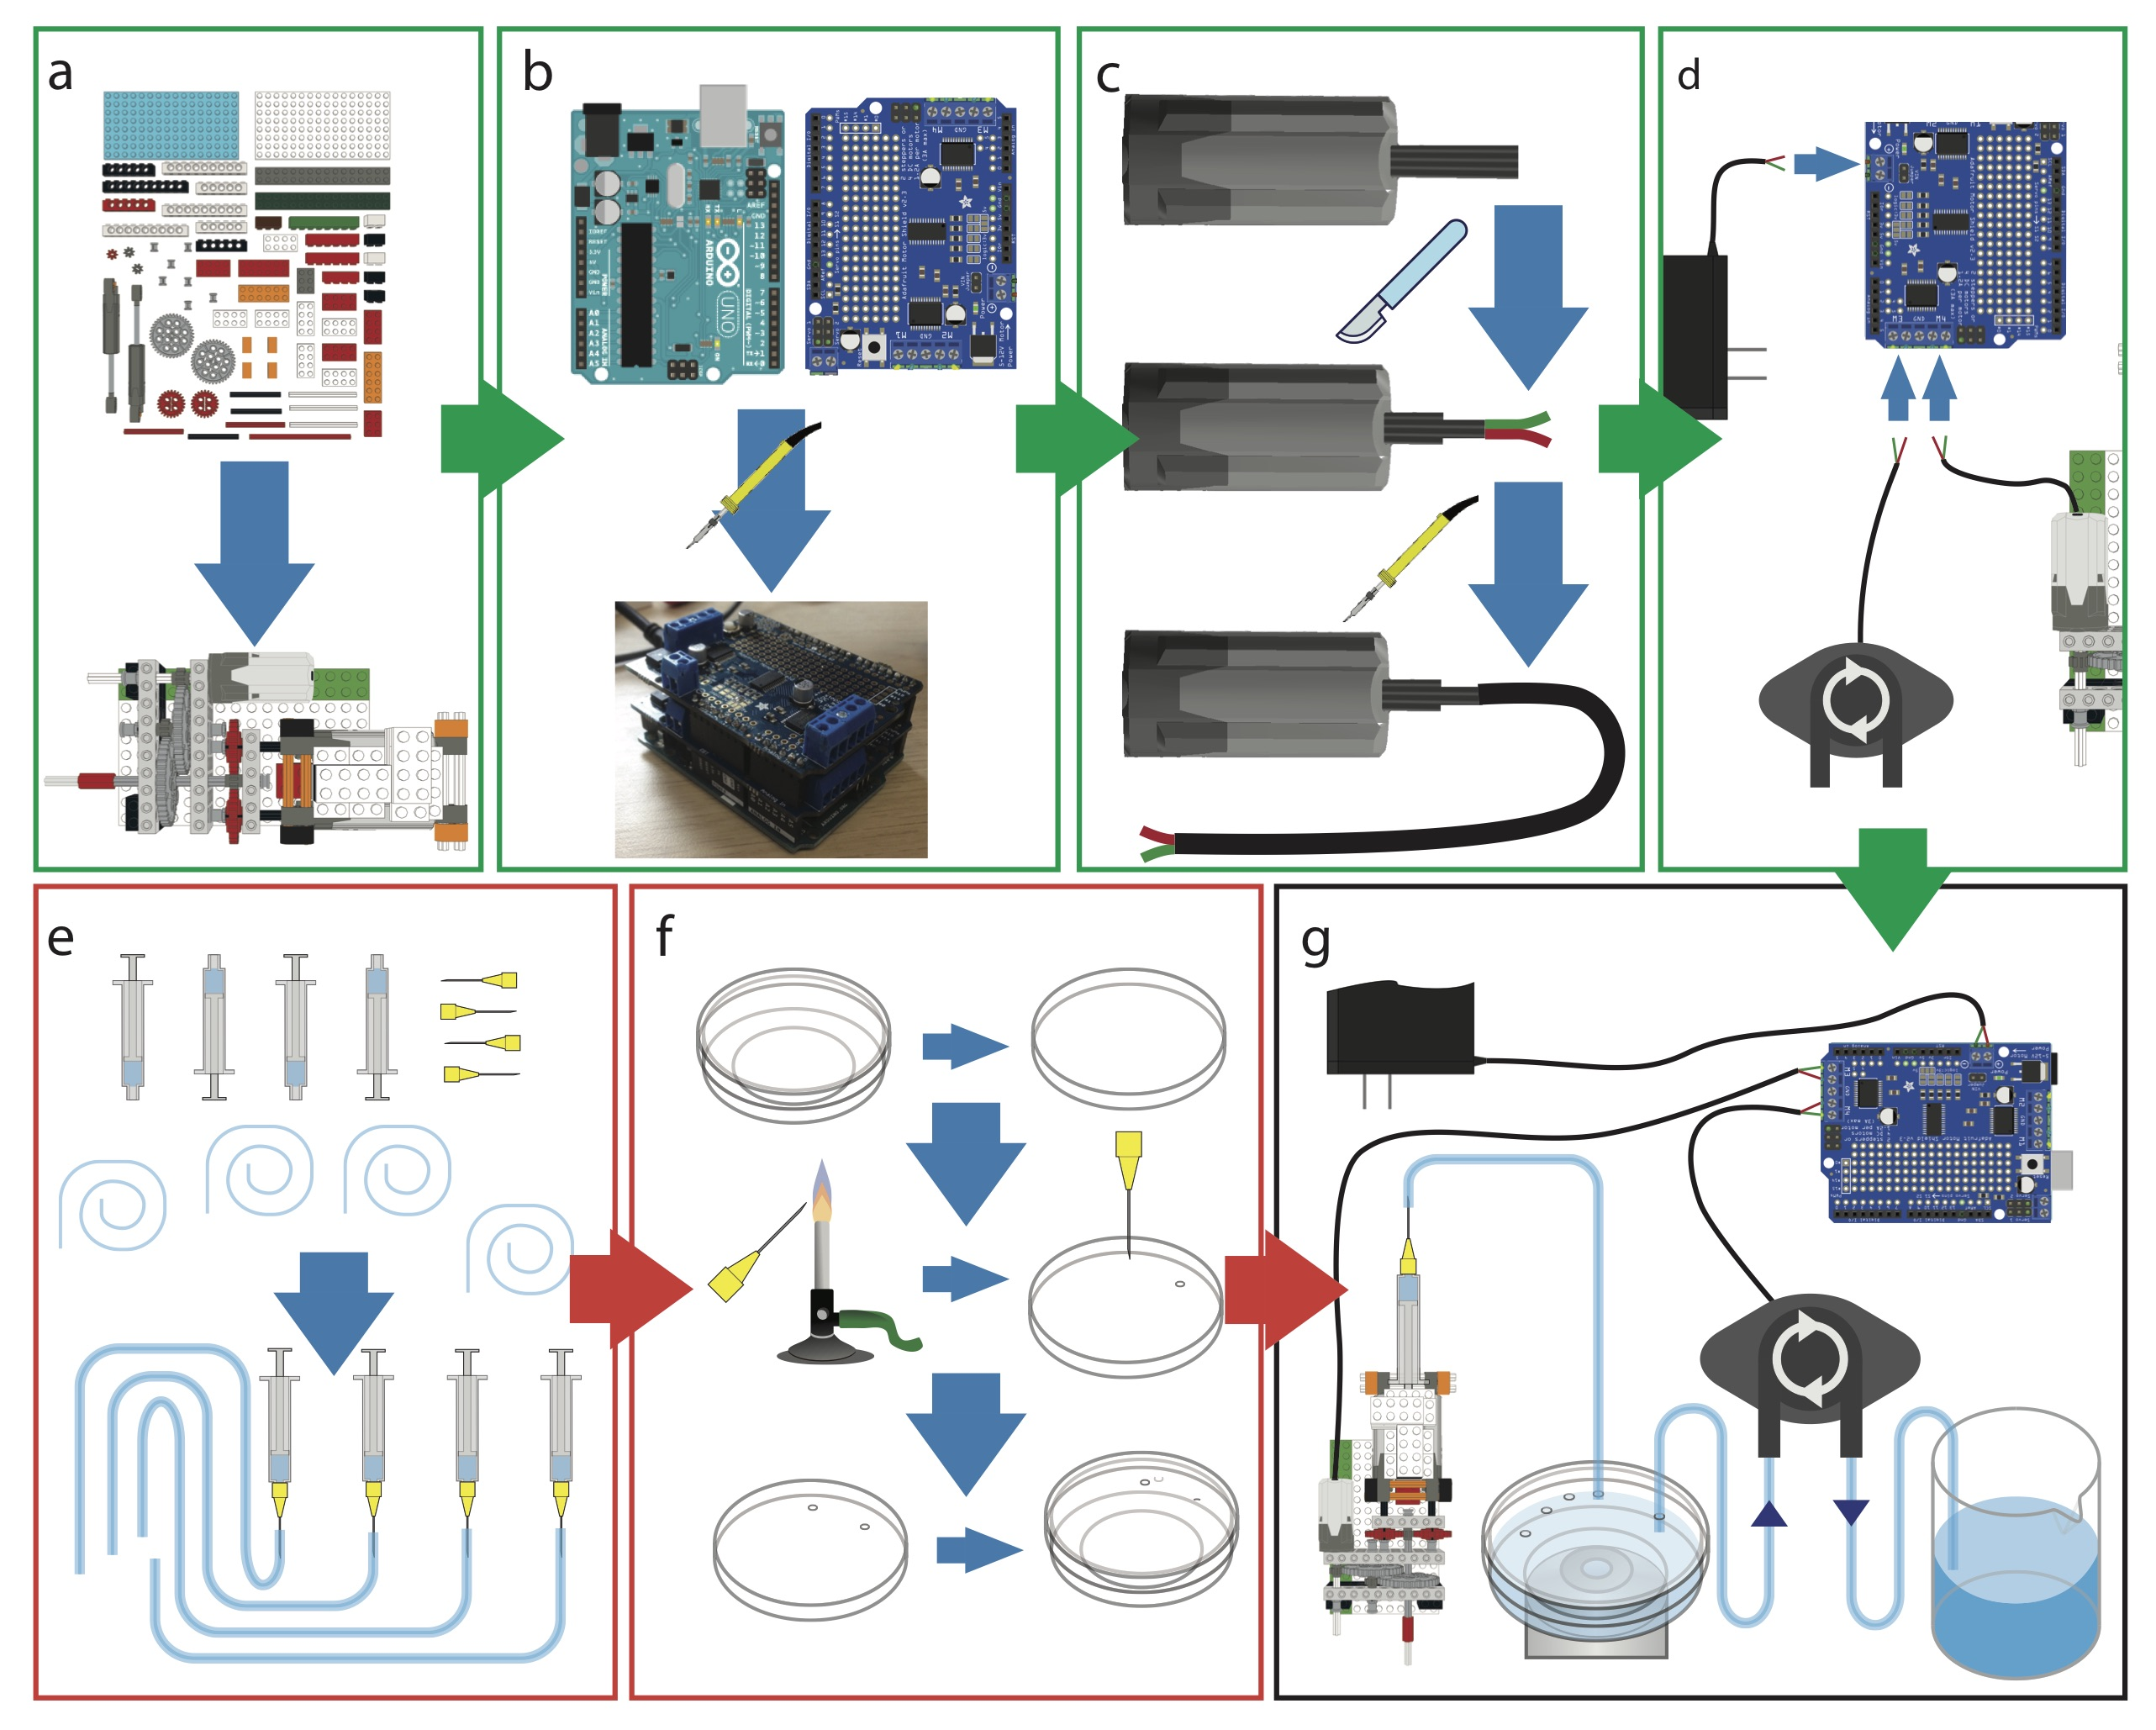
\includegraphics[width=\linewidth]{Figures/SFigure_Assembly}
%     \caption{\textbf{NanoJ-Fluidics pump assembly.} There are 4 steps to assemble a NanoJ-Fluidics system (a-d), and 2 steps to prepare an experiment (e,f). a) Build the syringe pumps from LEGO bricks. b) Assemble the electronic controller. c) Prepare the motor cables for wiring. d) Connect the pumps and power supply to the controller. e) Prepare the syringes. f) Prepare lid of the cell culture dish. g) Thread syringes on the dish lid and mount syringes on LEGO pumps.}
%     \label{supFig:PumpAssembly}
% \end{figure}
% %TC:endignore

% \vspace*{10pt}

% The NanoJ-Fluidics system is designed primarily for the sequential exchange of liquids in a glass-bottom cell culture dish (or equivalent supports, such as ATTOfluor coverlslip holders for example). It consists of several parts: LEGO based syringe pumps responsible for delivering reagents to the sample (Fig.~\ref{fig:PumpyDrawing}a and Fig. \ref{supFig:PumpAssembly}a); electronics responsible for controlling the pumps (Fig.~\ref{supFig:PumpAssembly}b-d); a peristaltic pump responsible for removing reagents from the sample (Fig.~\ref{fig:PumpyDrawing}b and Fig. \ref{supFig:PumpAssembly}d,g); fluid handling disposable components (Fig.~\ref{fig:PumpyDrawing}b and Fig.~\ref{supFig:PumpAssembly}e-f). The syringe pumps are designed to accommodate syringes of any size, to be cost-effective and simple to assemble. A syringe pump unit uses a simple gear and actuator system to convert the fast motor motion into a smooth and slower linear motion, to enable consistent fluid flow. The result is that the flow-rate will depend on the gears, motor speed and the syringe's internal diameter. The pumps can be calibrated by measuring the volume obtained at a given motor speed, syringe diameter and pumping time. Table \ref{supTable:syringeFlowRates} shows the volumes obtained with one pump after pumping for 10 seconds at maximum speed.

% \begin{table}[h!]
%     \centering
%     \begin{tabular}{ c | c | c | c | c }
%         Syringe Volume (mL) & Inner Diameter (mm) & Volume (\ce{\mu L})& Std. Dev. (\ce{\mu L}) \\
%         \hline
%         1 & 4.699 & 22.6 & 0.8  \\
%         5 & 8.7 & 134.71 & 5.8  \\
%         20 & 11.989 & 290 & 26.7  \\
%     \end{tabular}
%     \caption[Volumes obtained with BD Plastipak syringes]
%     {
%     Volumes obtained for BD Plastipak syringes of different sizes after pumping for 10 seconds at maximum speed. Std. Dev. is the standard deviation of volumes in 10 independent measurements. \\
%     }
%     \label{supTable:syringeFlowRates}
% \end{table}

% Both the syringe pump array (for media injection) and peristaltic pump (for media removal) are digitally run using an \href{https://www.arduino.cc/en/Guide/ArduinoUno}{Arduino UNO} micro-controller and \href{https://www.adafruit.com/product/1438}{Adafruit Motorshield} digital-to-analogue motor control. The Motorshield is an additional electronic board that connects to the top of the Arduino controller, enabling it to run up to 4 LEGO motors. An Arduino can be stacked with up to 32 Motorshields, limiting the controller to a maximum of 128 pumps, which should be sufficient for most NanoJ-Fluidics applications. We provide custom open-source firmware that enables the Arduino-based electronics to be programmatically controlled by a connected computer. We also provide a Java-based graphical user interface (GUI) for simple control of the fluidics sequences (Fig.~\ref{supFig:PumpAssembly}).\\

% The software interface can be set to automatically perform a sequence of liquid injection and liquid removal steps (Sup. Note Fig.~\ref{supFig:PumpSoftware}) allowing an entire sample fixation or labelling protocol to be carried as shown in Fig.~\ref{fig:LiveToFix}-\ref{fig:PAINT},~\ref{fig:Dix}.

% \subsection*{Assembly}
% \label{supnote:assembly}
% The steps to prepare a complete functioning NanoJ-Fluidics system (Fig. \ref{supFig:PumpOnScope} and \ref{supFig:PumpAssembly}) consist of assembling the pump array, controller, and wiring them together (Fig. \ref{supFig:PumpAssembly}a-d). Once the array and controller have been assembled, each experiment only requires the lab-ware component to be prepared anew (\ref{supFig:PumpAssembly}e-g). A full step-by-step guide for assembly and preparation can be found in \url{https://github.com/HenriquesLab/NanoJ-Fluidics/wiki}. \\

% NanoJ-Fluidics can also be used with more traditional microfluidics devices, such as Polydimethylsiloxane (PDMS) chips, however we have focused on providing a series of protocols using off-the-shelf labware (e.g. glass-bottom cell culture dishes). This approach makes the framework more accessible to laboratories that do not otherwise have the facilities to produce PDMS devices. When using culture dishes the primary use of the system is limited to liquid exchange, this effectively reproduces many laboratory protocols including cell fixation, immunolabeling, drug treatment, among others.

% %TC:ignore
% \begin{figure}[!ht]
%     \centering
%     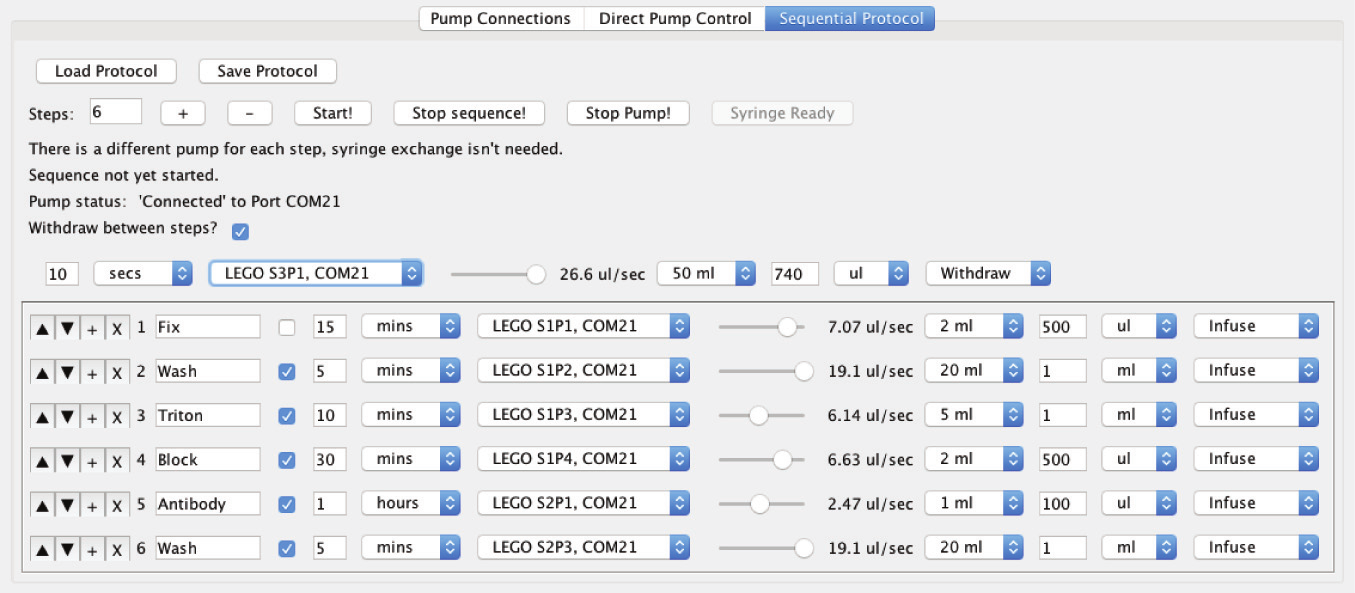
\includegraphics[width=\linewidth]{Figures/sFigureSoftware.png}
%     \caption{\textbf{User Interface.} Screenshot of the NanoJ-Fluidics sequential control user interface.}
%     \label{supFig:PumpSoftware}
% \end{figure}
% %TC:endignore

% \vspace*{10pt}

% \subsection*{Software interface and experiment automation} Control of the NanoJ-Fluidics pump array can be achieved in one of three ways: by using the provided Java-based GUI (Fig. \ref{supFig:PumpSoftware}); RS232 commands to the Arduino board; or by using the Application Programming Interface (API). A description of these is available at \url{https://github.com/HenriquesLab/NanoJ-Fluidics/wiki}.\\

% The RS232 command scheme enables researchers with programming experience to run the controller directly in their own software packages. However, the GUI was designed to enable any user to directly run any number of Arduino controllers and pumps, as well as design a sequence of steps associated to an experimental protocol (Fig. \ref{supFig:PumpSoftware}).\\

% NanoJ-Fluidics is controlled by a set of Java classes described in the API. For example, these can be used to enable a protocol generated in the GUI to be programmatically started and manipulated by outside applications, such as a microscope control software like Micro-Manager \cite{edelstein2014advanced}.

% %%%%%%%%%%%%%%%%%%%%%%%%%%%%%
% % Resolution characterisation
% %%%%%%%%%%%%%%%%%%%%%%%%%%%%%
% % ------------------------------------------------------------------------------------------------------------------------------------
% \newpage
% \section{Resolution mapping}
% % * <romain.cauk@gmail.com> 2018-04-23T12:33:11.755Z:
% % 
% % > olution mapping
% % This is not referred to in the text. What is the outcome of this FRC analysis? What conslclusions do you draw from this?
% % 
% % ^.
% \label{supnote:resolutionCharacterisation}

% %TC:ignore
% \begin{figure}[!ht]
%     \centering
%     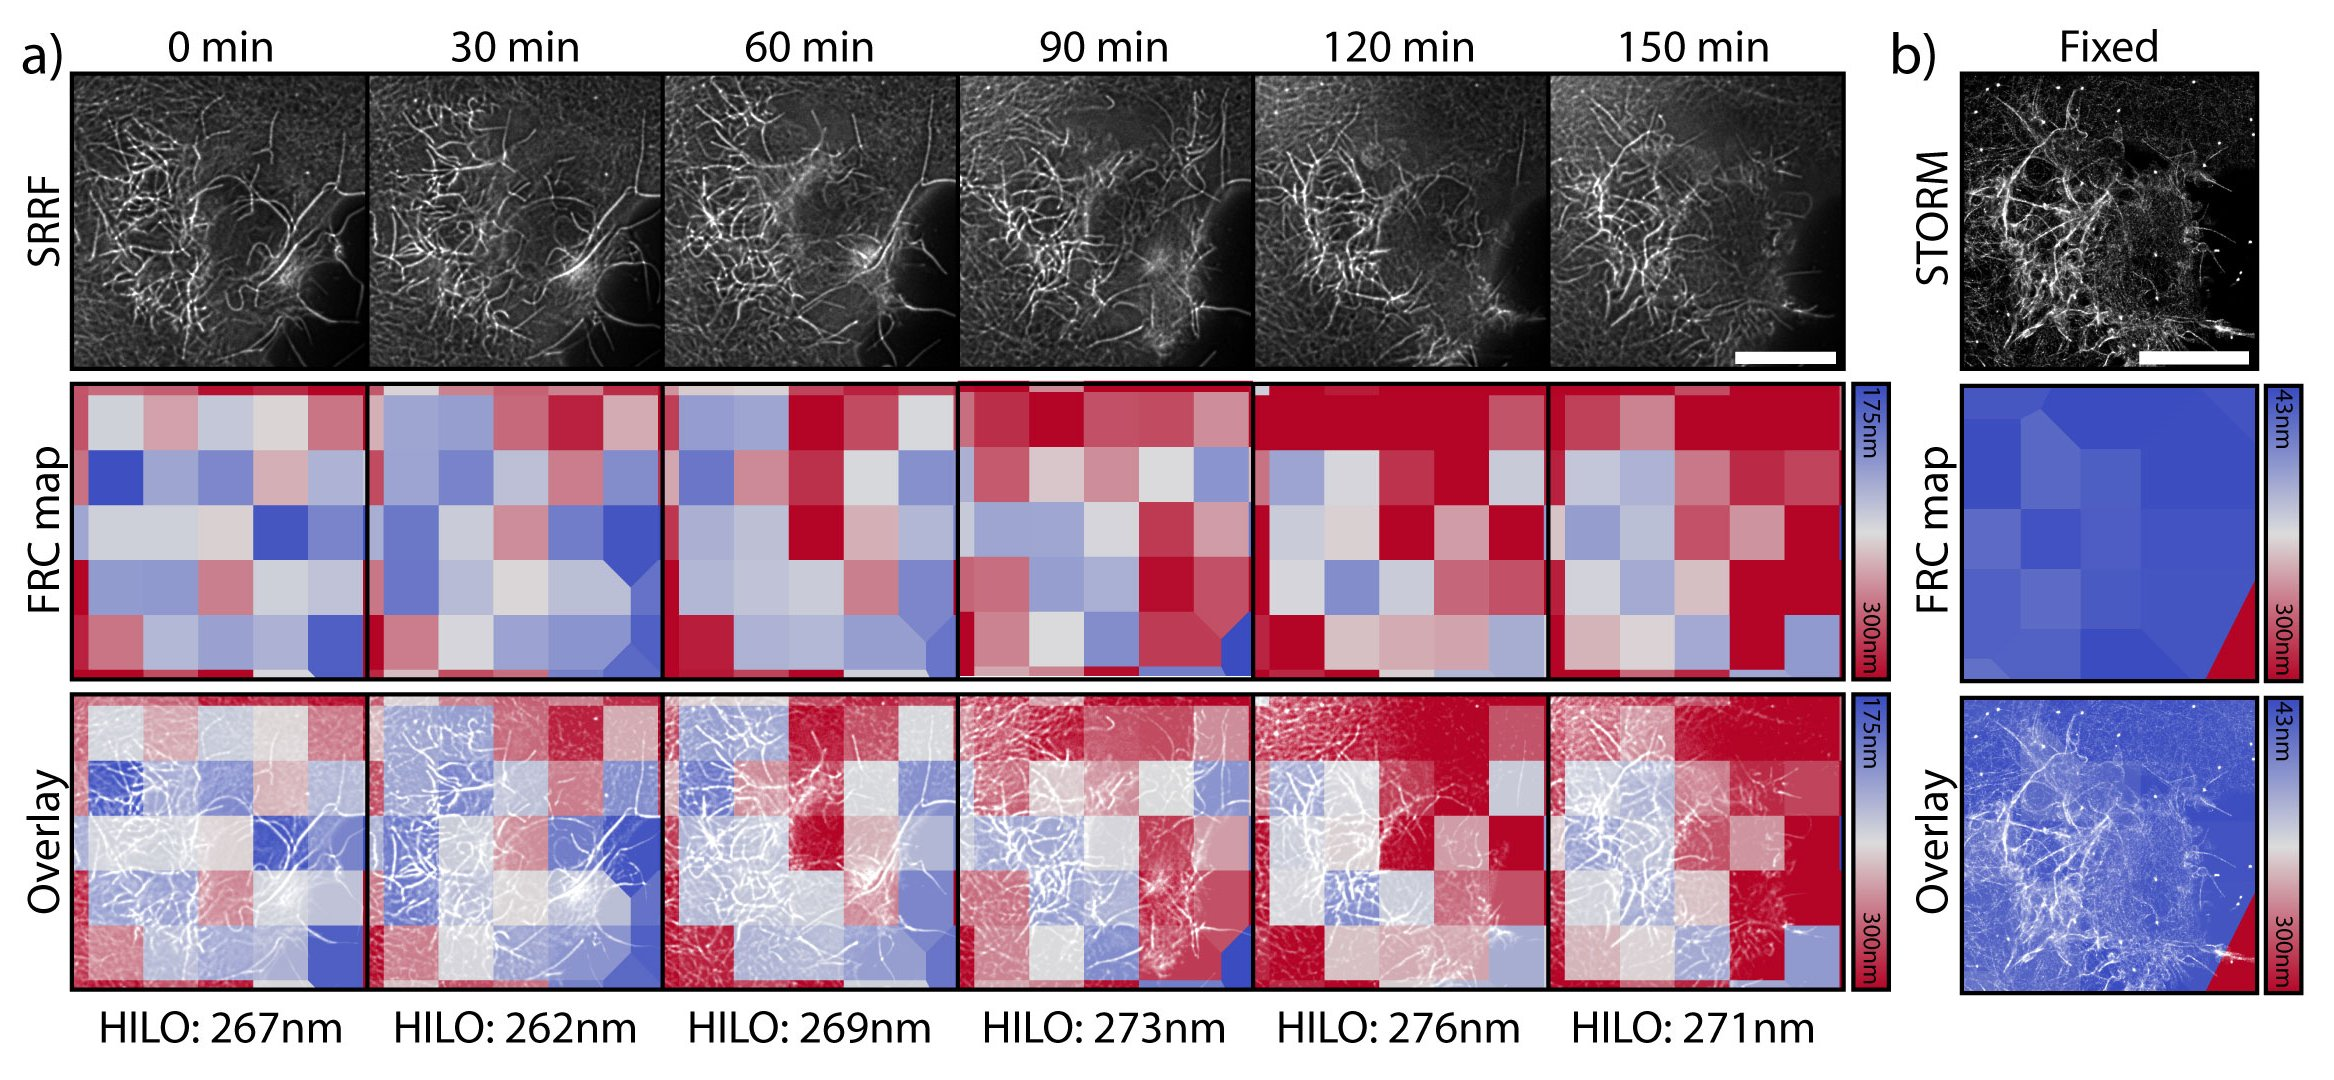
\includegraphics[width=.9\linewidth]{Figures/SFigure_FRC2}
%     \caption{\textbf{Fourier Ring Correlation (FRC) resolution mapping for Fig. \ref{fig:LiveToFix} and Sup. movie \ref{supmovie:live2fix} using NanoJ-SQUIRREL.} a) Individual live-cell SRRF frames at different time-points pre-fixation (top-row), equivalent FRC map (middle-row) and overlay between SRRF frames and the corresponding FRC map (lower-row); bottom values show average resolution calculated for the diffraction limited equivalent images. b) Individual STORM rendering acquired post-fixation (top); equivalent FRC map (middle); overlay between STORM frame and FRC map. Resolution maps calculated through NanoJ-SQUIRREL \cite{culley2018quantitative}. All scale bars are 10 \textmu{}m.}
%     % * <romain.cauk@gmail.com> 2018-04-23T12:27:26.957Z:
%     %
%     % > a) Individual SRRF frames at different time-points pre-fixation (top-row), equivalent FRC map (middle-row) and overlay between SRRF frames and the corresponding FRC map (lower-row); bottom values show average resolution calculated for the diffraction limited equivalent images. b) Individual \textit{d}STORM ren
%     % What is the point of the HILO values underneath each panel?
%     %
%     % ^.
%     \label{supFig:frcFig2}
% \end{figure}
% %TC:endignore

% %TC:ignore
% \begin{figure}[!ht]
%     \centering
%     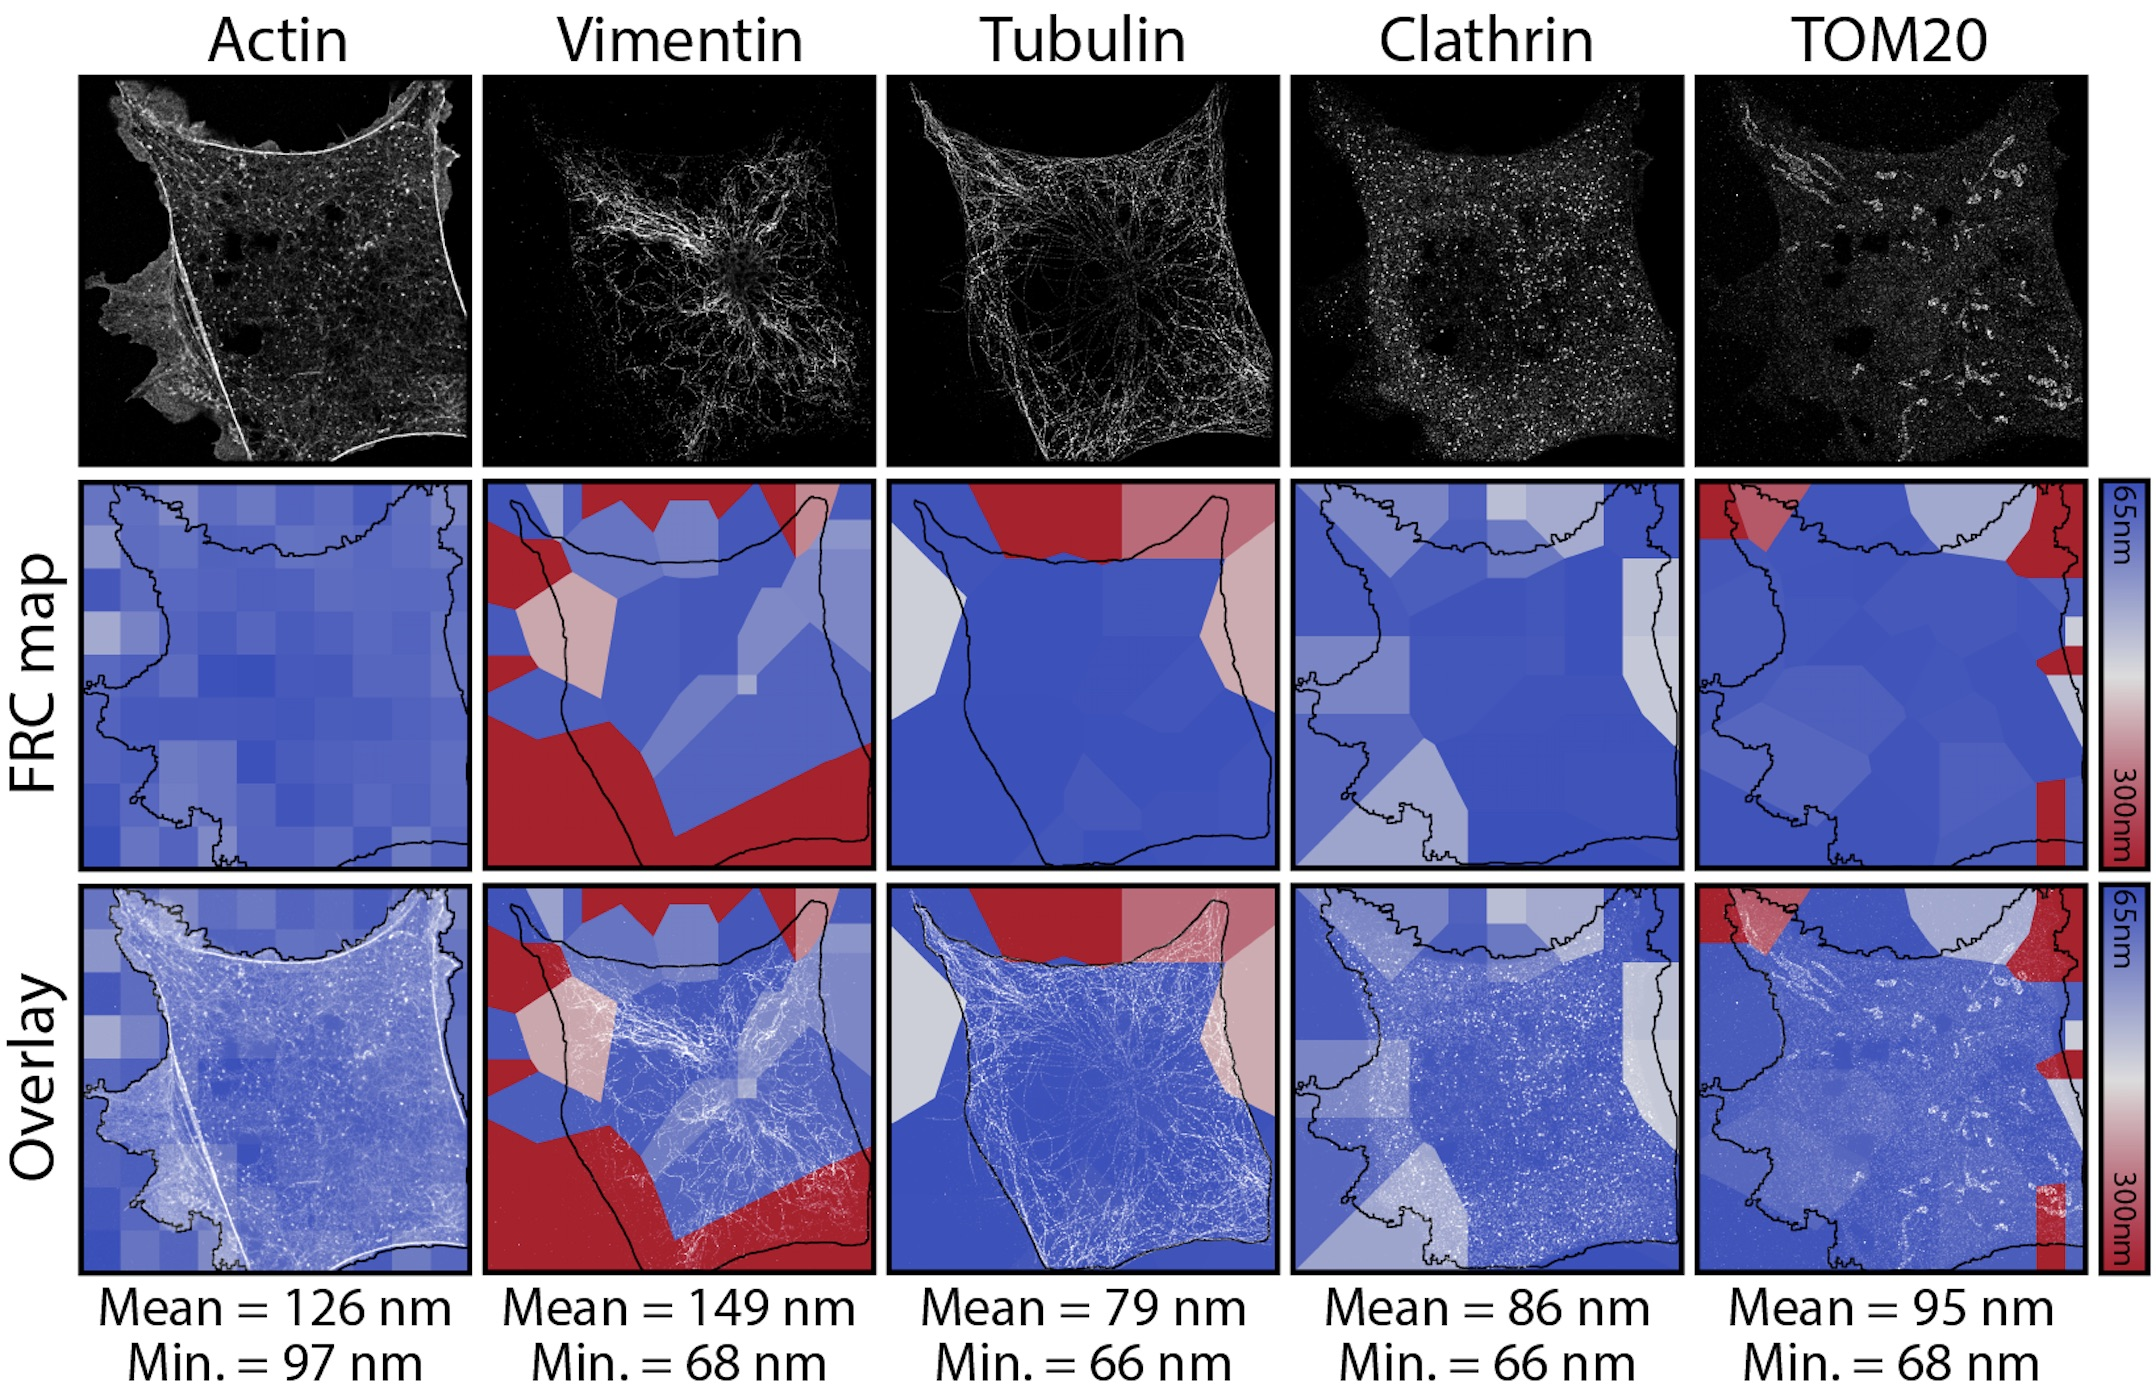
\includegraphics[width=.7\linewidth]{Figures/SFigure_FRC3}
%     \caption{\textbf{Fourier Ring Correlation (FRC) resolution mapping for Fig. \ref{fig:PAINT} and Sup. movie \ref{supmovie:multiplex} using NanoJ-SQUIRREL.} Individual DNA-PAINT super-resolution renderings (top-row), equivalent FRC map (middle-row) and overlay between SRRF frames and the corresponding FRC map (lower-row). Resolution maps calculated through NanoJ-SQUIRREL. Black outlines in middle and bottom rows indicate the cell shape mask used for calculation of mean and minimum resolutions across each channel.}
%     \label{supFig:frcFig3}
% \end{figure}
% %TC:endignore

% \vspace*{10pt}

% To estimate the local resolution achieved in the super-resolution renderings associated to the main figures, we carried out analysis using the Fourier Ring Correlation method \cite{nieuwenhuizen2013measuring}, recently modified in \cite{culley2018quantitative} to generate a resolution map. Fig. \ref{supFig:frcFig2} shows that the best resolution achieved for live-cell imaging with SRRF is 175nm, and 43nm for fixed-cell imaging with STORM. Fig. \ref{supFig:frcFig3} shows that the best resolution achieved in the DNA-PAINT channels is $\sim$67nm, with the exception of the actin channel which has an estimated best resolution of 97nm.

% %%%%%%%%%%%%%%%%%%%%%%%%%%%%%%%%%%%%%%%%%%%
% % Single colour live and fixed STORM imaging
% %%%%%%%%%%%%%%%%%%%%%%%%%%%%%%%%%%%%%%%%%%%
% % ------------------------------------------------------------------------------------------------------------------------------------
% \newpage
% \section{Nanoscale morphological changes between pre- and post-fixation}
% \label{supnote:changesFixation}

% %TC:ignore
% \begin{figure}[!ht]
%     \centering
%     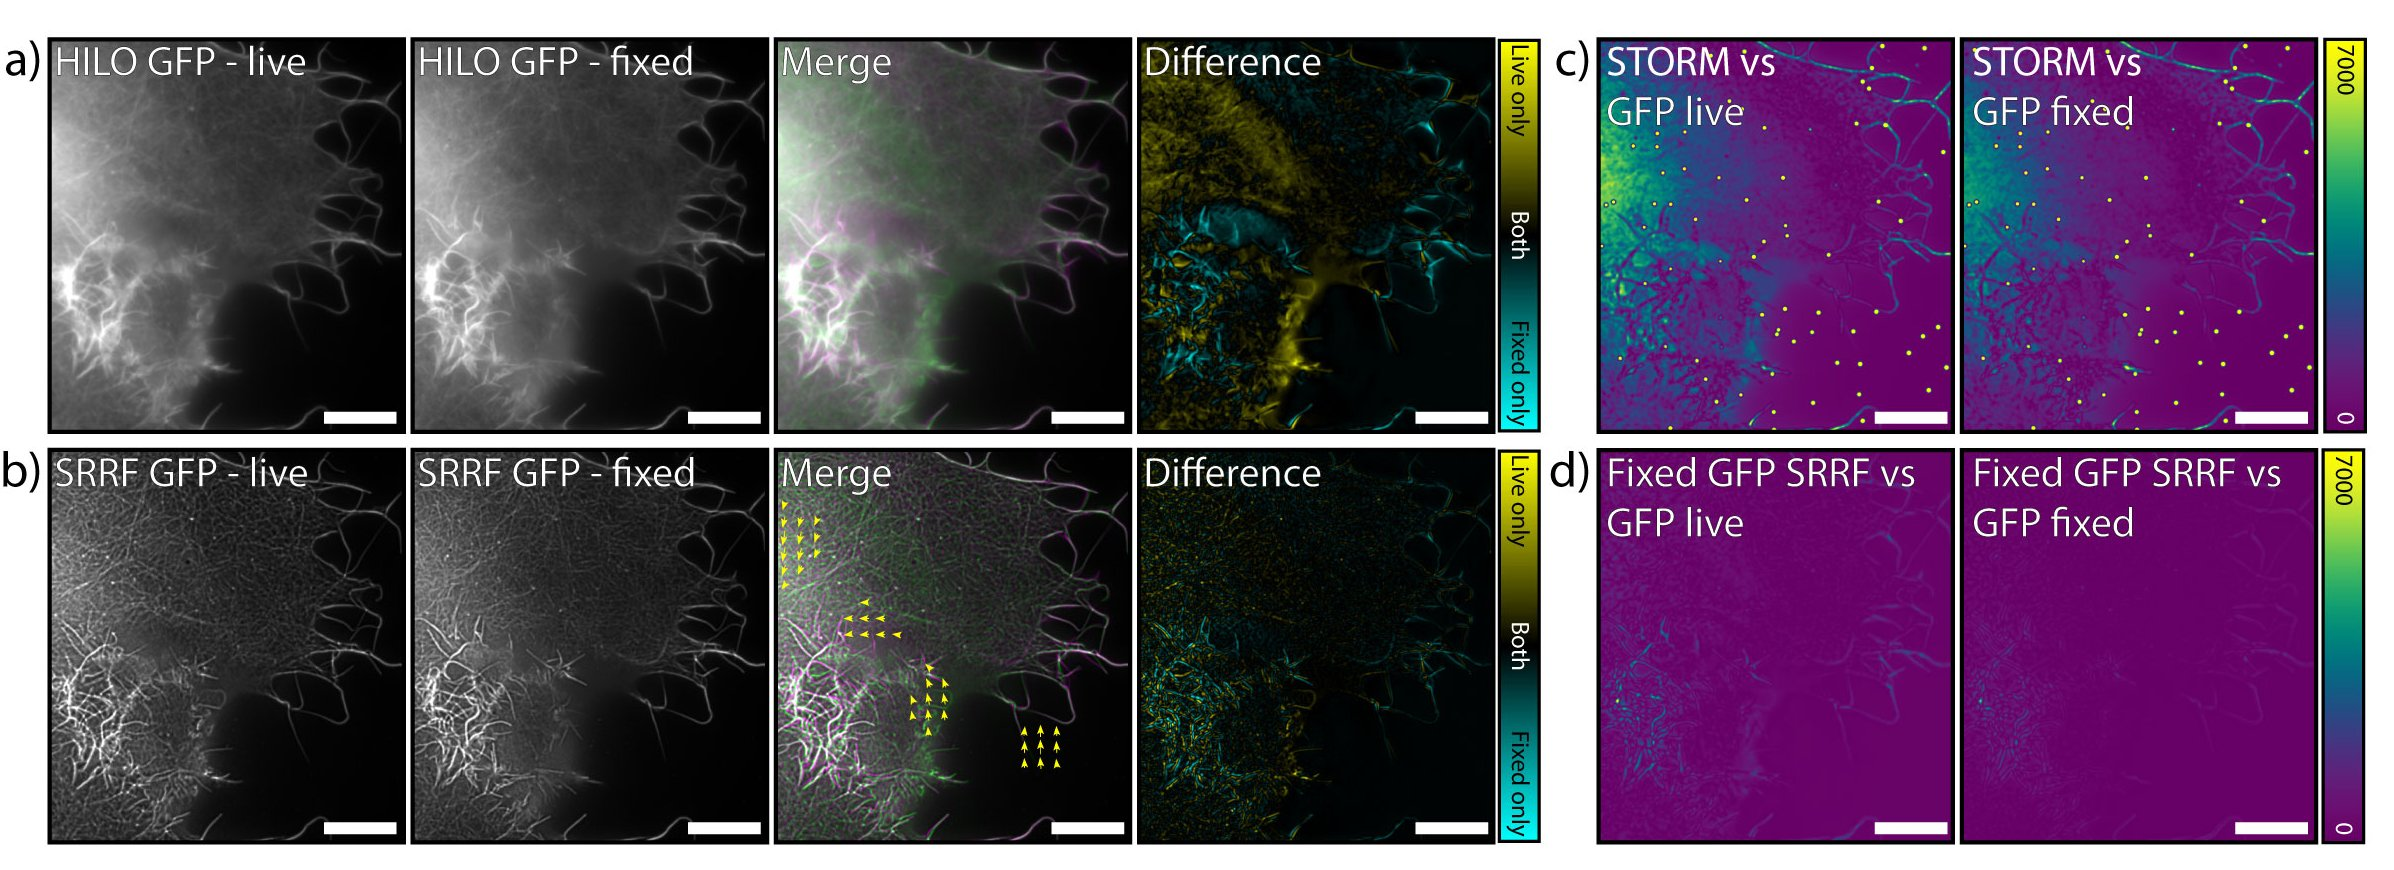
\includegraphics[width=\linewidth]{Figures/SFigure_CorrelationLive2Fix}
%     \caption{\textbf{Analysis of changes in cell morphology and labelling pre- and post-fixation.} a) Comparison of the distribution of GFP-labelled Utrophin in the cell shown in Fig. \ref{fig:LiveToFix} and Sup. movie \ref{supmovie:live2fix}, imaged in HILO. The last timepoint pre-fixation (`HILO GFP - live') and an image post-fixation of the same region (`HILO GFP - fixed') are shown. `Merge' shows an overlay of the live (green) and fixed (magenta) images. `Difference' shows the result of subtracting the fixed image from the live image. b) As in (a), except using the SRRF reconstructions of the data. The yellow arrows in `Merge' show parts of the cell which moved during fixation as measured using the elastic channel registration tool in NanoJ-SQUIRREL \cite{culley2018quantitative}. c) Error maps generated between the (fixed) STORM reconstruction of actin in this cell when using the live-cell GFP HILO image (left) or the fixed-cell GFP HILO image (right) as a reference. d) Error maps generated between the SRRF reconstruction of GFP in the fixed cell when using the live-cell GFP HILO image (left) or the fixed-cell GFP HILO image (right) as the reference. Scale bars = 10 \textmu{m}.}
%     \label{supFig:changesFixation}
% \end{figure}
% %TC:endignore

% \vspace*{10pt}

% To verify that there were no major alterations in cell morphology during fixation, we compared images of the same cell immediately before and after fixation. Fig. \ref{supFig:changesFixation}a shows pre- and post-fixation images for HILO imaging of the cell shown in Fig. \ref{fig:LiveToFix}, and Fig. \ref{supFig:changesFixation}b shows these changes for SRRF reconstructions of the same region. Overlaying both the SRRF and HILO images pre- and post-fixation shows that the morphology of the cell remains largely constant during fixation. There is movement of the bright filaments within the cell body and filopodia at the cell periphery on a sub-micron scale. This degree of movement is comparable to or smaller than the frame-to-frame movement shown in Sup. movie \ref{supmovie:live2fix}. There is also a loss of fluorescence intensity during fixation in the top left portion of the region shown in Fig. \ref{supFig:changesFixation}.\\

% %%%%%%%%%%%%%%%%%%%%%%%%%%%%%%%%%%%%%%%%%%%
% % Fixation-on-event imaging
% %%%%%%%%%%%%%%%%%%%%%%%%%%%%%%%%%%%%%%%%%%%
% % ------------------------------------------------------------------------------------------------------------------------------------
% \newpage
% \section{Event-driven fixation imaging}
% \label{supnote:Fixation-on-event}

% NanoJ-Fluidics has also the advantage of allowing sample treatments, such as fixation, at precise times during the experiment. Thanks to the integration of NanoJ-Fluidics with the image acquisition, determining the time of treatment can be triggered by imaging cues. To demonstrate this capacity, we carried out an experiment observing the state of focal adhesions, as mammalian cells progress into division. Fixation was triggered by the observation of the rounding of the cells as they approach mitosis \cite{ramkumar2016coupling}. Also, in order to fully exploit the fluidics automation of NanoJ-Fluidics, we combined it with tiling imaging and image stitching in order to obtain fields-of-view of several millimetres while preserving high resolution.

% \begin{figure*}[!b]
%     \centering
%     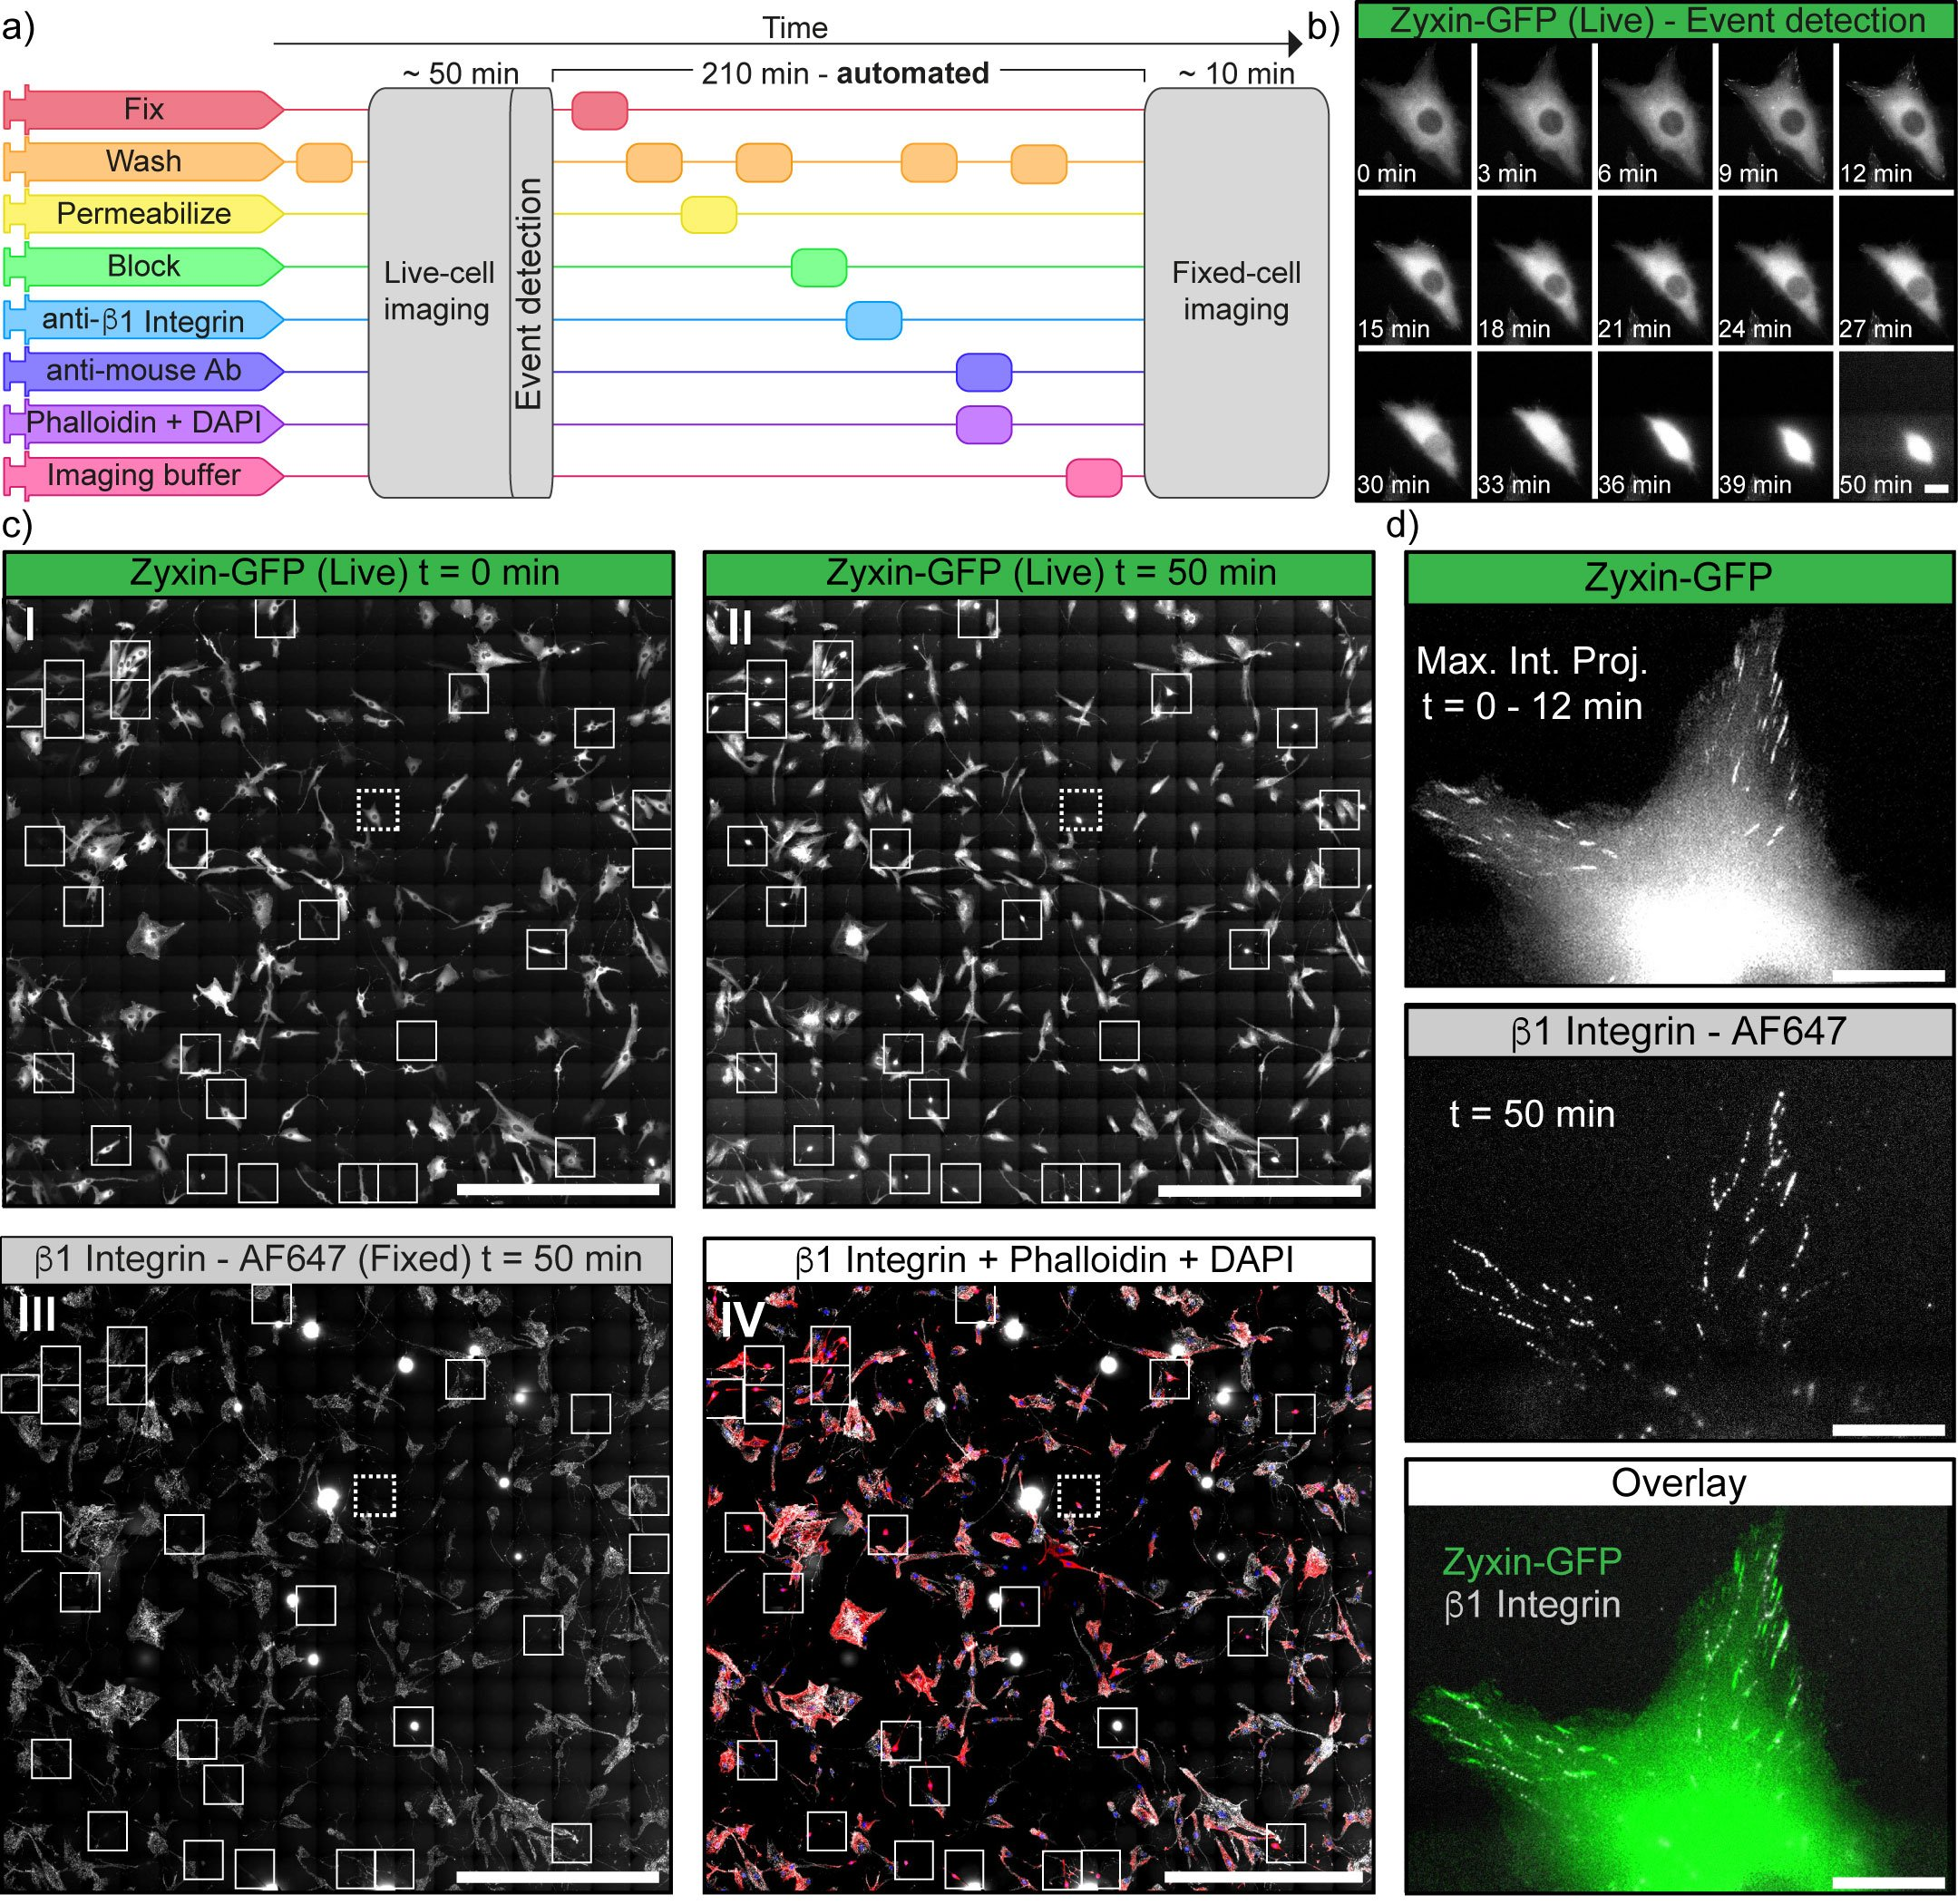
\includegraphics[width=\textwidth]{Figures/Figure_Sxx_Dix}
%     \caption{\textbf{Event-driven fixation of cells upon mitotic rounding} a) NanoJ-Fluidics workflow of the  event-driven protocol performed. b) Stills of RPE1 zyxin-GFP live-cell time-lapse during mitotic rounding. Scale bar, 20 \textmu{}m. c) Stitched mosaic (17x17 individual regions) of: I- First frame of the live-cell time-lapse; II- Last frame of the live-cell time-lapse; III- RPE1 zyxin-GFP cells immunolabelled for active β1-integrin; IV- Overlay of RPE1 zyxin-GFP cells immunolabelled for active β1-integrin and stained for F-actin (with phalloidin-TRITC) and DNA (with DAPI). Insets represent cells where mitotic rounding was observed (Sup. Movie \ref{supmovie:dix}), dashed inset is the cell in b) and d). Scale bar is 1 mm. d) I - Maximum intensity projection of the first 12 min in b); II - Active β1-integrin staining; III - Overlay of both panels. Scale bar, 20 \textmu{}m.}
%     \label{fig:Dix}
% \end{figure*}

% We first blocked asynchronous cells in G2 via treatment with a CDK1 inhibitor (RPE1 cells expressing zyxin-GFP). Next, the cell cycle was released by exchanging the inhibitor by growth media using NanoJ-Fluidics (Fig. \ref{fig:Dix}a) and imaged by live-cell time-lapse microscopy (Fig. \ref{fig:Dix}b). When the observed cells reached a minimal area (an indicator of mitotic rounding), the fixative was injected (Fig. \ref{fig:Dix}a-b). A considerable portion of cells ($\sim$10\%) were found to be fixed in a similar rounding state due to the simultaneous release of the G2 block (insets of Fig. \ref{fig:Dix}c I, Sup. Movie \ref{supmovie:dix}). The sample was then immunolabelled for β1-integrin, plus co-stained for F-actin and DNA, then imaged (Fig. \ref{fig:Dix} c III-VI). Both actin and DNA staining allowed a secondary visual validation of pre-mitotic cell rounding. As we recently described using comparable experiments~\cite{dix2018role}, β1-integrin is shown to retain a similar spatial pattern similar to zyxin when the cells were spread on the substrate, in their pre-division shape (Fig. \ref{fig:Dix}d). We observed that, while zyxin retracts during cell rounding (Fig. \ref{fig:Dix}b), β1-integrin remains in its original position (Fig. \ref{fig:Dix}d and Sup. Movie \ref{supmovie:dix}), helping guide daughter cell migration \cite{dix2018role}.


% %%%%%%%%%%
% % Movies %
% %%%%%%%%%%
% \newpage
% \setcounter{figure}{0} % reset figure counter for Sup. Figures
% \renewcommand{\figurename}{Movie}

% \newpage
% \begin{figure}[!ht]
%     \centering
%     %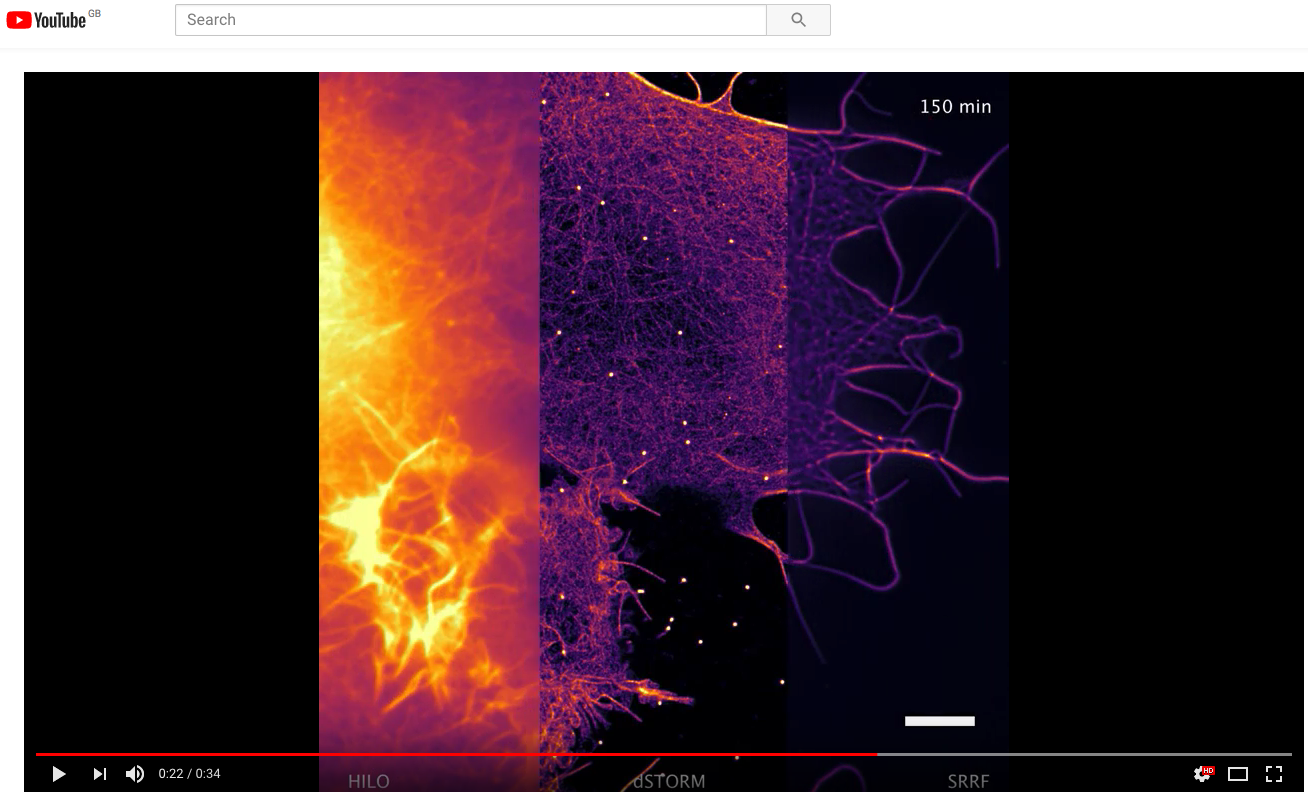
\includegraphics[width=0.8\linewidth]{Figures/Screen_Shot_SMovie1}
%     \caption{\textbf{Live-to-Fix Super-Resolution Imaging with NanoJ-Fluidics.} Movie corresponding to Fig. \ref{fig:LiveToFix}. HILO and HILO-SRRF live imaging of transiently transfected COS7 cells expressing UtrCH-GFP. After live-imaging the same cells were fixed and stained with phalloidin-AF647 for STORM imaging. All steps were performed using the NanoJ-Fluidics syringe pump array without taking the sample from the microscope. Scale bars correspond to 10 \textmu{}m.}
%     \label{supmovie:live2fix}
% \end{figure}

% \newpage
% \begin{figure}[!ht]
%     \centering
%     %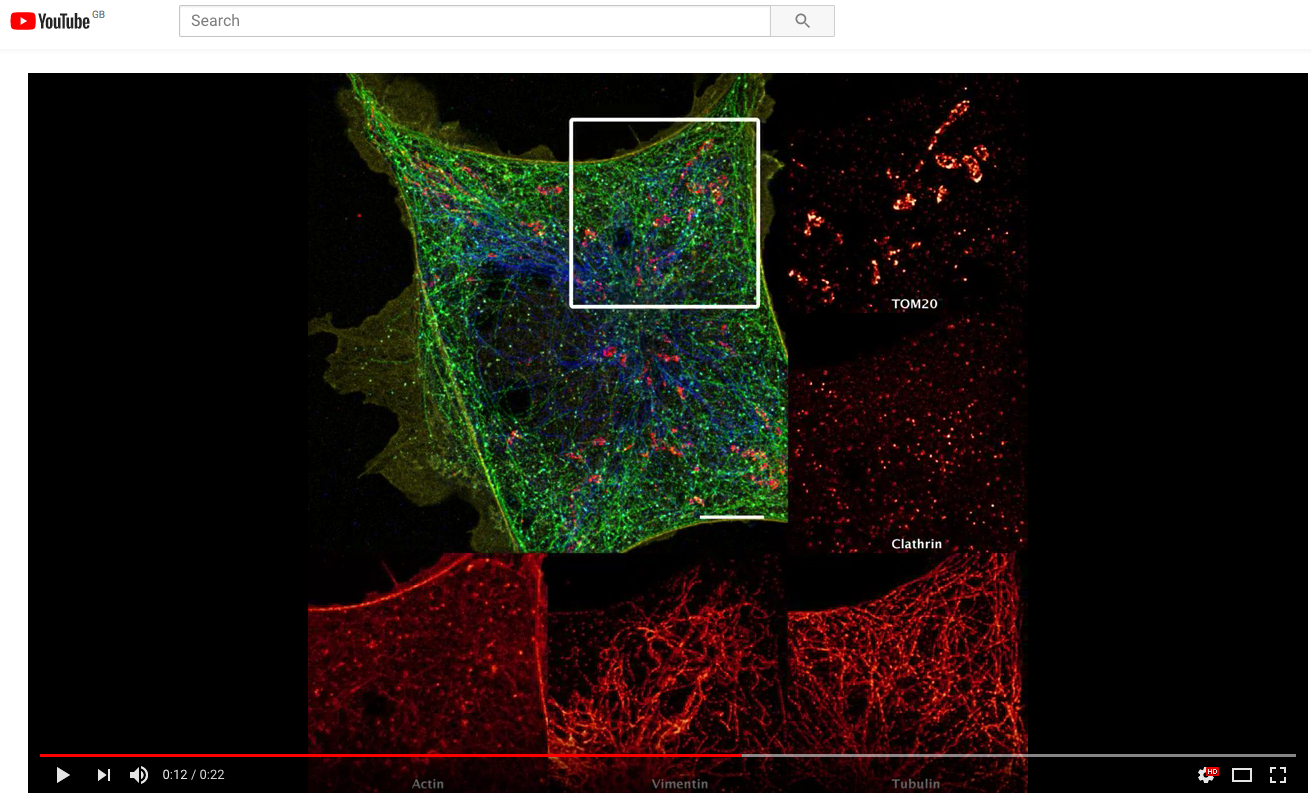
\includegraphics[width=0.8\linewidth]{Figures/Screen_Shot_SMovie2}
%     \caption{\textbf{Automated Multiplex Super-Resolution with NanoJ-Fluidics.} Movie corresponding to Fig. \ref{fig:PAINT}. STORM imaging of COS7 cells stained with phalloidin-Atto488, and DNA-PAINT imaging of vimentin, TOM20, tubulin and clathrin the same cell. Imaging buffer exchange steps were performed using the NanoJ-Fluidics syringe pump array directly on the microscope stage. Scale bars corresponds to 10 \textmu{}m.}
%     \label{supmovie:multiplex}
% \end{figure}

% \newpage
% %TC:ignore
% \begin{figure}[!ht]
%     \centering
%     %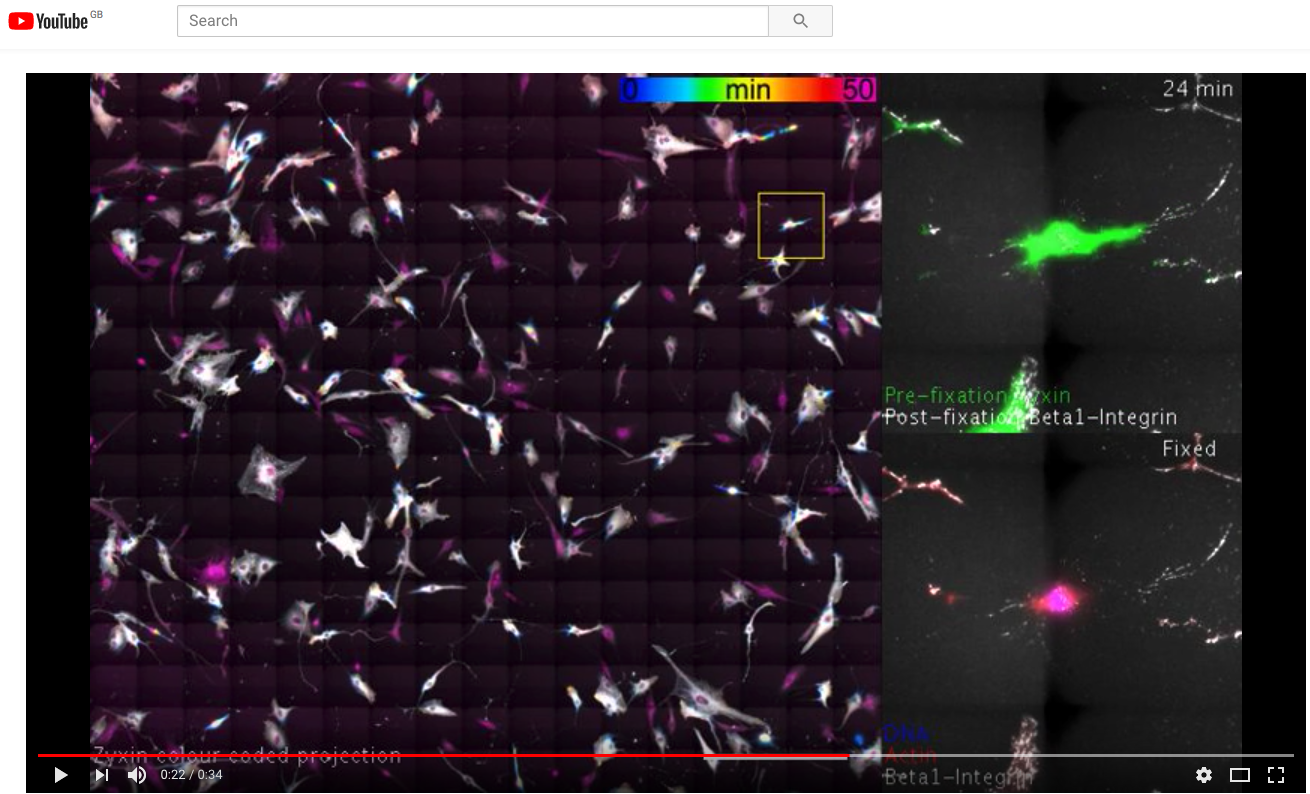
\includegraphics[width=0.8\linewidth]{Figures/Screen_Shot_SMovie3}
%     \caption{\textbf{Event-driven live-to-fixed imaging with NanoJ-Fluidics.} Movie corresponding to Fig. \ref{fig:Dix}. Left: colour coded time projection of a stitched mosaic (17x17 individual regions), following RPE1 cells stably expressing zyxin-GFP undergoing mitotic rounding. Upon enough cells rounded (event detection) cells were fixed and immunolabelled for active β1-integrin and stained for actin and DNA. On the top right corner, overlay of zyxin-GFP in live cells with active β1-integrin after fixation. First and last regions correspond to cells not undergoing mitotic rounding, whereas all remaining regions display RPE1 cells rounding and showcase the colocalization of active β1-integrin (post-fixation staining) with focal adhesions (zyxin-GFP). Bottom right corner, overlay of active β1-integrin, phalloidin and DAPI staining after fixation. Scale bar corresponds to 0.5 mm.}
%     \label{supmovie:dix}
% \end{figure}
% %TC:endignore


% % ------------------------------------------------------------------------------------------------------------------------------------
% % ------
% % Bibliography
% % ------
\newpage
\section*{Supplementary Bibliography}
\bibliographystyle{zHenriquesLab-StyleBib}
\bibliography{06_Bibliography_Clean}